\documentclass[12pt,a4paper]{article}

\usepackage[T1]{fontenc}
\usepackage{amsmath, amssymb, amsfonts}
\usepackage[magyar]{babel}
\usepackage[utf8]{inputenc}
\usepackage{graphicx}
\usepackage{graphics}
\usepackage{mathtools}
\usepackage{epsfig}
\usepackage{epstopdf}
\usepackage{cite}
\usepackage{caption}
\usepackage{hyperref}
\usepackage[bottom=4cm]{geometry}
%\geometry{a4paper, portrait, margin=1in}

\title{\huge{Korszerű vizsgálati módszerek labor jegyzőkönyv}\\ \vspace{20pt}
\textbf{Kalorimetria}}

\author{\Large{\textsc{Csörnyei Géza}} \vspace{10pt}\\
	\textrm{Eötvös Loránd Tudományegyetem}\\
	\textrm{Fizika BSc III. évfolyam}
	}
\date{}
%\lhead{}
\begin{document}
\addtolength{\voffset}{-1.0cm}
\addtolength{\textheight}{1.0cm}
\begin{titlepage}
\maketitle

\begin{figure}[!htb]
\centering

\includegraphics[scale=0.6]{eltecimer.jpg}
\end{figure}

\hfil \Large{'C' mérőcsoport}\hfil  \\
\vspace*{2pt}
\hfil \Large{\emph{Mérés dátuma:} 2018.05.14.}\hfil \\
\vspace*{2pt}
\hfil \hspace*{45pt} \Large{\emph{Mérés vezetője:} Groma István}\hfil
\thispagestyle{empty}
\end{titlepage}

\section{Bevezetés}

\hspace*{10pt} Mérésünk során a hőeffektussal járó folyamatok vizsgálatához használt kalorimetriával ismerkedtünk meg. Több különböző anyag esetén megvizsgáltuk az olvasztás folyamatát, majd kiértékeltük a kaloriméter által kapott eredményeket, ezzel meghatározva a kívánt termodinamikai mennyiségeket.

\section{Rövid elméleti összefoglaló}
 
\hspace*{10pt} A méréseinkhez egy DSC (\emph{Differential Scanning Calorimeter}) eszközt használtunk. Ezen műszerben a minták (referencia és mérendő) külön mintatartókban foglalnak helyet, külön fűtjük fel őket. A DSC-ben két visszacsatoló kör is található: az egyik a két minta átlaghőmérsékletét hivatott a beállított sebesség szerint növelni, a másik pedig a két minta hőmérsékletének függvényében csökkenti illetve növeli az egyes mintákat fűtő kályhák teljesítményeit, ezzel elérve, hogy a program szerinti melegítés közben a két minta hőmérsékletének különbsége egyre kisebb lesz. A DSC műszer közvetlenül a teljesítményt méri, mely a visszacsatolások miatt arányos lesz a két anyag hőmérsékletének különbségével.\\
\hspace*{10pt} A kaloriméter által mért teljesítmény, feltételezve, hogy a kaloriméter relaxációs ideje elhanyagolható, az alábbi összeg formájában áll elő:
\begin{equation}
w=(c_m - c_r )v+\frac{dh}{dt} + w_{bas}(T),
\end{equation}
ahol $c$-k a minta, illetve a referenciaanyag fajhői, $h$ az entalpia, $w_{bas}(T)$ pedig az alapvonal, mely egy számunkra ismeretlen, a minta és a kaloriméter által befolyásolt függvény. A kalorimetriában ezen alapvonalnak a meghatározása jelenti a legnagyobb problémát, ez befolyásolja a mérések pontosságát. Az alapvonal meghatározására numerikusan van lehetőség, de gyakorta szükség van kézi beavatkozásokra, mivel viselkedését nem minden esetben lehet pontosan leírni a programoknak.\\
\hspace*{10pt} A mérések során reverzibilis és irreverzibilis folyamatokkal is találkozhatunk. Általában úgy lehet kiszűrni az irreverzibilis folyamatokat, hogy a fűtést leállítva hagyjuk lehűlni a mintát az átalakulás hőmérséklete alá, majd újra felfűtjük, ezáltal a második esetben csak a reverzibilis folyamatot kapva.  A szétválasztás automatizálásához modulálhatjuk a kályhák hőmérsékletét egy meghatározott periodikus felfűtéssel, így a fűtés kikapcsolása nélkül el tudjuk választani az irreverzibilis folyamatot a reverzibilisektől.\\
\hspace*{10pt} Termikusan aktivált folyamatoknak nevezzük azon folyamatokat, melyek során a kezdetben egy lokális szabadentalpia minimumban levő rendszer csupán a termikus fluktuációk hatására egy másik minimumba kerül. Ilyen folyamatok esetében az aktiválási energia meghatározásához az alábbi formulát kell használnunk:
\newpage
\begin{equation}
\ln (v) = a-1.052 \frac{Q}{R}\frac{1}{T_{max}},
\end{equation}
ahol $v$ a fűtési sebesség, $a=a(Q,Z,n)$ paraméter, $Q$ a folyamat aktiválási energiája, $R$ az univerzális gázállandó, $n$ a folyamatra jellemző paraméter, $T_{max}$  a fázis koncentrációjának időbeli változásának maximumához tartozó hőmérséklet.

\section{Mérési eredmények kiértékelés}
\subsection{Indium minta olvasztása}
\hspace*{10pt} Mérésünket egy indium minta olvasztásával kezdtük. Az alapvonal megszerkesztése és levonása után a laborban használt programmal egyenest illesztettünk a felfutási szakaszra, majd az ábrára rajzolt két jel között kiszámoltuk a görbe, azaz a csúcs területét. Az egyenesillesztésből a tengelymetszet, így az olvadáspont értéke $T=429.75$ K, míg a csúcs területe, az olvadáshő  $L=-27.148$ J/g. A kapott értékek jó közelítéssel megfelelnek az irodalmi értékeknek [1]:\\ $T_{ir}=429.7$ K és $L_{ir}=28.6$ J/g.\\
\begin{figure}[!h]
\centering
  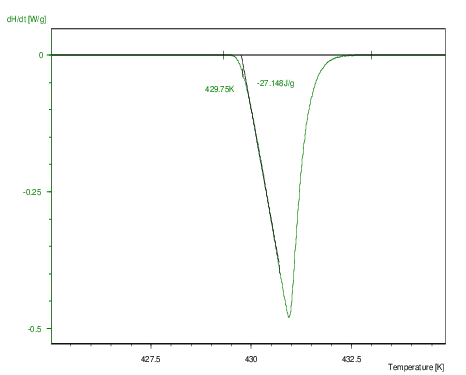
\includegraphics[width=0.8\linewidth]{2fin}
\caption{Az indium minta melegítése során kapott görbe (az alapvonal levonása után) és annak kiértékelése}
\end{figure}
\newpage

\subsection{Sn-Pb minta olvasztása}
\hspace*{10pt} A mérés során használt ötvözet egy eutektikus ötvözet, azaz létezik olyan ötvözőarány, mely egy adott, jól meghatározható olvadásponttal rendelkezik. Mérésünk során az ezen esethez tartozó koncentrációtól egy kicsit eltérő arányú ötvözéssel készült mintát használtunk. Ahogy az a \ref{fig:snpb}. ábrán is látható, nem volt egyenes az illesztett alapvonal. Ennek oka, hogy az eltérő fázisok eltérő fajhőkkel rendelkeznek. Az alapvonal illesztése és levonása után, amint az az ábráról is leolvasható, az átalakulási hőmérsékletekre $T_{szol}=455.36$ K és $T_{likv}=537.36$ K-t kaptunk, míg az olvadási hőre $L=-26.883$ J/g-ot kaptam. Egy az interneten talált ([2]) fázisdiagram alapján ez a minta kb. 75 m/m$\%$ Pb-t tartalmazott.
\begin{figure}[!h]
\hspace*{-20pt}
\minipage{0.5\textwidth}
  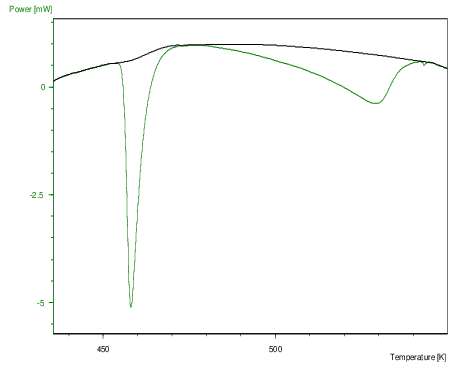
\includegraphics[width=\linewidth]{3fin}
\endminipage
\hspace*{10pt}
\minipage{0.5\textwidth}
  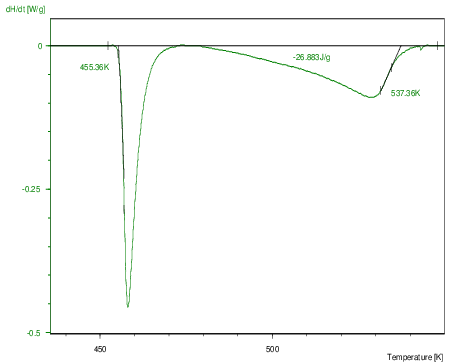
\includegraphics[width=\linewidth]{4fin}
\endminipage
\caption{Sn-Pb ötvözet vizsgálata}
\label{fig:snpb}
\end{figure}
\newpage
\subsection{Fémüveg átkristályosodása}
\hspace*{10pt} A mérés során következő lépésként a fémüveg átkristályosodását, mint termikusan aktivált folyamatot vizsgáltuk meg. Az aktiválási energia meghatározásához három különböző fűtési sebességgel végeztük el a mérést (40 K/min, 20 K/min és 10 K/min). Mivel az első sebesség esetén a mérés még gyorsan történt, ezért ott két felfűtést végeztünk, mivel az átkristályosodás egy irreverzibilis folyamat. A pontosság érdekében el kellett volna végeznünk ezt a másik két sebesség esetén is, azonban erre nem volt elegendő a laborgyakorlat alatt rendelkezésünkre álló idő. A kapott termogrammokat a \ref{fig:megnincs}. ábrán lehet megtekinteni. A termogrammokról leolvasható hőmérsékletértékeket a \ref{tab:üveg}. táblázatban foglaltam össze. A kapott adatokra a \ref{egyenes}. egyenlet szerint egyenest illesztettünk. Az illesztés a \ref{egyenes}. ábrán látható.
\begin{table}[!h]
\begin{center}
\begin{tabular}{|c|c|}
\hline
$v$ [K/min] & $T_{\textrm{max}}$ [K] \\
\hline
\hline
10 & 661.39 \\
\hline
20 & 670.60 \\
\hline
40 & 680.44 \\
\hline
\end{tabular}
\caption{A mért $T_{max}$ értékek az egyes fűtési sebességek esetére}
\label{tab:üveg}
\end{center}
\end{table}

\begin{figure}[!h]
\centering
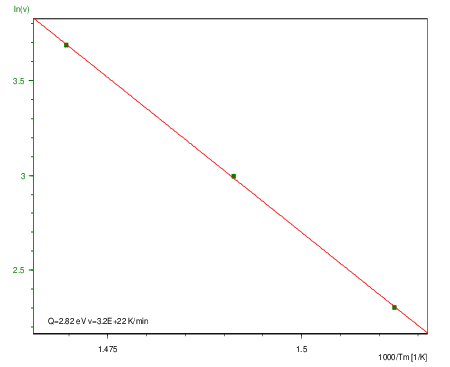
\includegraphics[width=0.8\linewidth]{12fin}
\caption{Az $\ln v - 1/T_{\textrm{max}}$ összefüggés szerint illesztett egyenes}
\label{egyenes}
\end{figure}

\newpage
\begin{figure}[!htb]
\hspace*{-20pt}
\minipage{0.5\textwidth}
  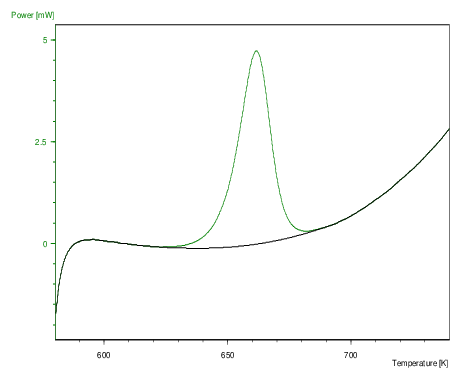
\includegraphics[width=\linewidth]{10fin}
\endminipage
\hspace*{10pt}
\minipage{0.5\textwidth}
  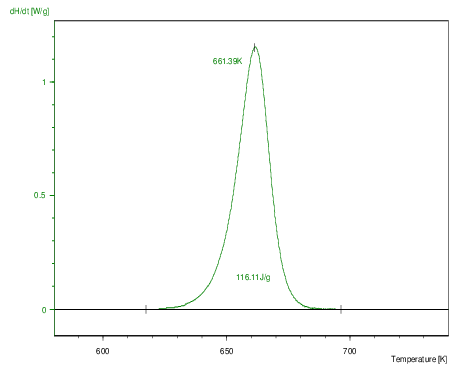
\includegraphics[width=\linewidth]{11fin}
\endminipage
\\
\hspace*{-20pt}
\minipage{0.5\textwidth}
  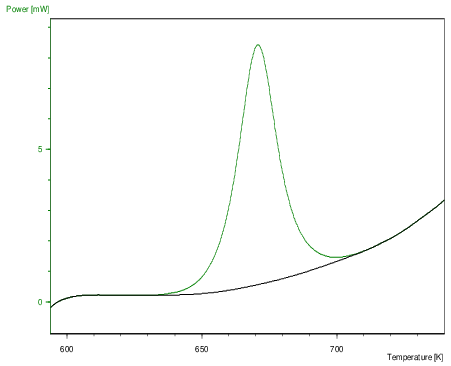
\includegraphics[width=\linewidth]{8fin}
\endminipage
\hspace*{10pt}
\minipage{0.5\textwidth}
  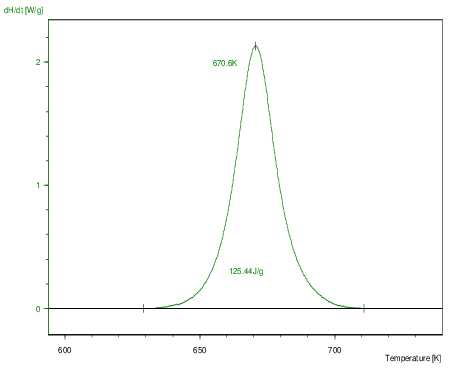
\includegraphics[width=\linewidth]{9fin}
\endminipage
\\
\hspace*{-20pt}
\minipage{0.5\textwidth}
  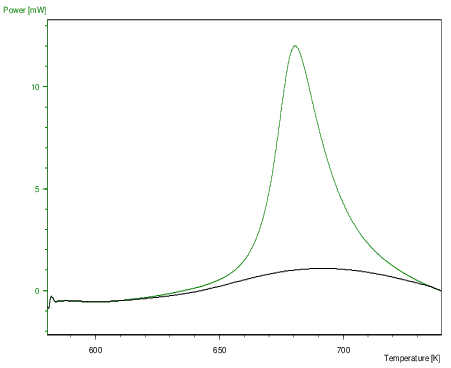
\includegraphics[width=\linewidth]{6fin}
\endminipage
\hspace*{10pt}
\minipage{0.5\textwidth}
  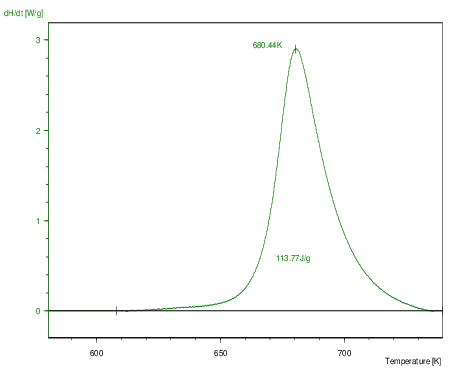
\includegraphics[width=\linewidth]{7fin}
\endminipage
\caption{Rendre 10, 20 és 40 K/mind fűtési sebességek mellett kapott görbék, valamint a kiegyenesített alapvonal feletti csúcs esetén mért entalpiaváltozások, valamint $T_{max}$ hőmérsékletek}
\label{fig:megnincs}
\end{figure}
A mérési pontokra illesztett egyenes meredekségéből meg lehetett határozni az anyag aktiválási energiáját, amely így $Q=2.82$ eV-nak adódott.
\newpage
\subsection{Ni fázisátalakulása}
\hspace*{10pt} A Ni fázisátalakulásának vizsgálatához moduláltuk a fent említett módon a fűtést. Ekkor a kapott jel átlaga jó közelítéssel az irreverzibilis folyamatokat, míg az amplitúdó a reverzibilis folyamatokat tükrözte. Egy ilyen módon készített adatsor látható a \ref{fig:ni}. ábrán.\\
\begin{figure}[!h]
\centering
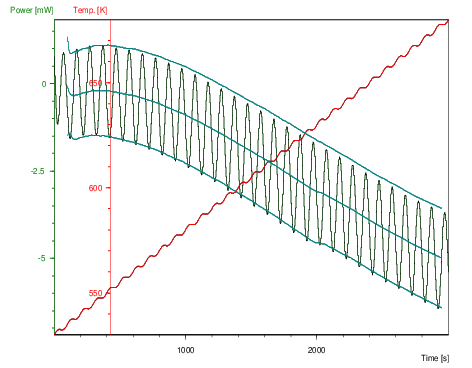
\includegraphics[width=0.7\linewidth]{13fin}
\caption{A Ni mintán végzett modulált mérés}
\label{fig:ni}
\end{figure}


\hspace*{10pt} A mérésből kapott fajhő idő-, illetve hőmérsékletfüggése a \ref{fig:fajho}. ábrán látható. Itt a fázisátalakulás csúcsa jelenik meg, amely a mérés alapján $T_c = 625.51$ K-nek adódott, ezzel szemben az interneten fellelt ([3]) irodalmi érték 631 K.

\begin{figure}[!h]
\hspace*{-20pt}
\minipage{0.5\textwidth}
  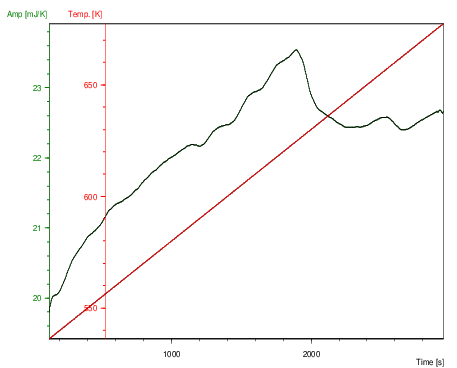
\includegraphics[width=\linewidth]{14fin}
\endminipage
\hspace*{10pt}
\minipage{0.5\textwidth}
  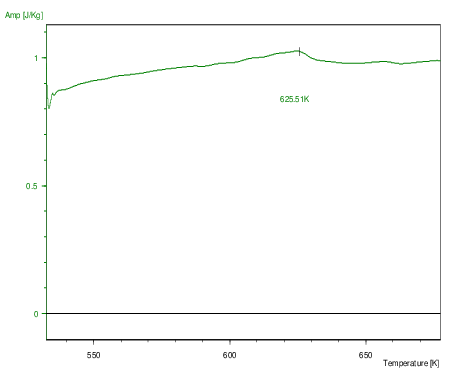
\includegraphics[width=\linewidth]{15fin}
\endminipage
\caption{A Ni minta fajhőjének változása az idő és a hőmérséklet függvényében}
\label{fig:fajho}
\end{figure}

\section{Diszkusszió}
\hspace*{10pt} Mérésünk során megismerkedtünk a kalometriai mérésekhez szükséges berendezésekkel, valamint több mintán is sikeres méréseket végeztünk, a kapott eredmények jól tükrözték az irodalmi értékeket.

\section*{Hivatkozások}
\hspace*{14pt} [1] : \texttt{https://en.wikipedia.org/wiki/Indium}\\
\hspace*{14pt} [2] : \texttt{https://upload.wikimedia.org/wikipedia/\\ \hspace*{84pt} commons/d/d6/Diagramme$\_$binarie$\_$Pb$\_$Sn.svg}\\
\hspace*{14pt} [3] : \texttt{https://hypertextbook.com/facts/2005/StephanieMa.shtml}
\end{document}